\documentclass[12pt,letterpaper]{report}
\usepackage{natbib}
\usepackage{geometry}
\usepackage{fancyhdr}
\usepackage{afterpage}
\usepackage{graphicx}
\usepackage{amsmath,amssymb,amsbsy}
\usepackage{dcolumn,array}
\usepackage{tocloft}
\usepackage{asudis}
\usepackage{multirow}
\usepackage{lmodern}
\usepackage[pageanchor=true,plainpages=false,pdfpagelabels,bookmarks,bookmarksnumbered]{hyperref}
\usepackage{subcaption}

\begin{document}
%-----------------------front matter
\pagenumbering{roman}
\title{Characterization of Energy and Performance Bottlenecks in \newline Omnidirectional Camera Systems}
\author{Sridhar Gunnam}
\degreeName{Master of Science}
\paperType{Thesis}
\defensemonth{July}
\defenseyear{2018}
\gradmonth{July}
\gradyear{2018}
\chair{Prof. Robert LiKamWa}
\memberOne{Prof. Pavan Turaga}
\memberTwo{Prof. Suren Jayasuriya}

\maketitle
\doublespace
\begin{abstract}

Generating real-world content for VR is challenging in terms of capturing and processing at high resolution and high frame-rates. The content needs to be captured for a truly immersive experience where the user can look around in 360-degree view and perceive the depth of the scene. The existing solutions only capture and offloading the compute load to the server. But offloading large amounts of raw camera feeds takes longer latencies and poses difficulties for real-time applications.  By capturing and computing on the edge, we can closely integrate the systems and optimize for low latency, but moving the traditional stitching algorithms to battery constrained device needs at-least three orders of reduction in power. We believe that close integration of capture and compute stages will lead to synergies in terms of reduced capture, interface, and compute power. 

We approach the problem by building a hardware prototype and characterize the end-to-end system bottlenecks like power and performance. The prototype has 6 IMX274 cameras and uses Nvidia Jetson TX2 development board for capture and computation. We found that capturing is bottlenecked by sensor power and data-rates across interfaces, whereas compute by the total number of computations per frame. Our characterization shows that redundant capture and redundant computations lead to high power, huge memory footprint, and high latency. The existing systems lack hardware-software co-design aspects leading to excessive data transfers across the interfaces and expensive computations within the individual subsystems. We finally propose mechanisms to optimize the system for low power and low latency. We emphasize the importance of co-design of different subsystems to reduce and reuse the data. For example, reusing the motion vectors of the ISP stage reduces the memory footprint of the stereo correspondence stage. Our estimates show that pipelining, parallelizing on custom FPGA can achieve low latency for real time stitching.
 	
\end{abstract}

\dedicationpage{}
\begin{acknowledgements}
		I would like to thank my advisor Prof. Robert Likamwa for his continuous support and guidance. He helped shape my ideas and made me confidant to work in ambiguities. I would like to thank my mom Sujatha and dad Peddakapu, brother Raghu, and late grandma Bhanumathi for their eternal love and support.	I would like to thank Monish Pabrai and Dakshana, who played a crutial role when I was looking for opportunities in school. 	I thank my friends Kotta, Palanki, Gadda, Raks, Pathre and Penju for  the moral support whenever needed in US. I would like to thank my flatmates KV, TR, Vivek Rai, and Deshpande, and my friends Druthi, and lab buddies Jinhan, Venky, Siddhant, Vraj, Alireja, Paul, and Saad. I especially thank Sahab for his willingness to help others. Most of all I would like to thank Abbu Tataya for his belief in me and supporting me financially. I thank Shanthi pinni and Hari Babi for being supportive to my family during tough times.  
	
%	I would also like to thank brother Raghu,  cousins Naveen, Chinnu, Lavu, Mahesh, and my dearest sis Reshu, fun cousins Sunny, Teja, Akhi, Nikkhi, and uncle Muralidhar Rao, Rambabu, Srinu, Vijay Babai. I would also like to thank my bava Babby, akka Lakshmi for their love. 

\end{acknowledgements}
\tableofcontents
% This puts the word "Page" right justified above everything else.
\addtocontents{toc}{~\hfill Page\par}
% Asking LaTeX for a new page here guarantees that the LOF is on a separate page
% after the TOC ends.
\newpage
% Making the LOT and LOF "parts" rather than chapters gets them indented at
% level -1 according to the chart: top of page 4 of the document at
% ftp://tug.ctan.org/pub/tex-archive/macros/latex/contrib/tocloft/tocloft.pdf
\addcontentsline{toc}{part}{LIST OF TABLES}
\renewcommand{\cftlabel}{Table}
\listoftables
% This gets the headers for the LOT right on the first page.  Subsequent pages
% are handled by the fancyhdr code in the asudis.sty file.
\addtocontents{lot}{Table~\hfill Page \par}
\newpage
\addcontentsline{toc}{part}{LIST OF FIGURES}
\addtocontents{toc}{CHAPTER \par}
\renewcommand{\cftlabel}{Figure}
% This gets the headers for the LOF right on the first page.  Subsequent pages
% are handled by the fancyhdr code in the asudis.sty file.
\addtocontents{lof}{Figure~\hfill Page \par}
\listoffigures
%-----------------------body
\doublespace
\pagenumbering{arabic}
\chapter{Introduction}

With the advent of AR/VR technologies there is an increasing demand to capture real world content for immersive viewing experience. The real world content needs to be captured from cameras and then processed to the format in which the content can be viewed in AR/VR. The main characteristics of this content is to provide immersive seamless experience where user can view in any direction as if they were teleported to that location. In order to have such immersive experiences, we need to bridge the gaps in several domains including optics, graphics, audio and video, etc. But during this project we focus on capture systems for 360 degree video. \newline

What does it means to have capture visually immersive real world scenes? Researchers \cite{cuervo2018creating} predict that we need very high resolution(16k) and framerates(120+) to make the experience visually indistinguishable from reality. Current 360 stereo video systems are used mainly designed for professional videography. They consist of several camera(18 in google's jump VR \cite{richardt2017video}) which are bulky, and capture lot of data which will is offloaded and used to generate AR/VR videos thereby limiting their usability. But in order to easily capture and share such experiences we need also need to focus on usability and portability of the devices to make 360 video mainstream in AR/VR.

We increase the usability and portability of the 360 devices if we can capture and stitch the panorama on the same devices. Most of the software uses traditional algorithms fit for offloading based approaches and doesn't consider power budget for implementing 360 capture using a low power portable device. 
360 video is essential for VR, but capturing and stitching videos in real-time is limited by battery life. In-order to tackle the challenge of capturing and stitching on the same device, we study the system level bottlenecks in energy and performance by building a prototype. We characterize the system level bottlenecks in terms of performance per watt and latency. %[ [[condense this]
Our findings suggest that the main reason for the inefficiency is caused by building the system from off the shelf camera and traditional stitching algorithms. Conventional 360 degree video is captured using a multi-camera rig and the expensive stitching is offloaded to powerful machines. Although some systems exist where stitching is done online, they are limited by output resolution, framerate and battery life. We show that the inefficiencies in the pipeline are due to lack of hardware algorithm co-design. In this paper we study the data flow of the stitching pipeline by building a prototype using 6 camera system. We analyze the energy and performance bottlenecks in the pipeline and analytically evaluate the proposed optimizations. 
 
% Although commercial 360 degree solutions exist, they are mostly used for capture and stitching is offloaded to powerful machines. This limits the usability of 360 in VR and also portability and for heating. Our goal is therefore to build a 360 camera system that optimizes the entire pipeline both in hardware and software. We characterize the traditional pipeline and propose
%------------------------------

%Characterizing monoscopic, stereoscopic, bottlenecks, optimization

The document is organized as follows, in chapter two we discuss about the background and related work describing the general stitching pipeline for VR panorama generation. In chapter three we present the evaluation results of the prototype system design. We then discuss proposed optimizations in chapter four, and conclude in chapter five.

The contributions of our work are as follows:\newline
1) Build end-to-end system for capturing 360 degree video.\newline
2) Characterize individual stage power and performance and highlight the bottlenecks in the system.\newline
3) Propose architectures to optimize end-to-end data flow and data abstractions needed at sub-system level, i.e, optimizing the spatio-temporal redundancies in the capture and computation.\newline % Intro
\chapter{Background}
Existing systems \newline
Google Jump, Facebook Surround, Mega Stereo, Samsung Gear 360 \newline
Differentiating our work \newline
Bottlenecks in the existing systems \newline

Data Flow \newline
Block Diagram
- With different stages
- With Data Inputs and Data Outputs of each stage. (Zoom in Diagram) % Background
\chapter{Characterization}

Our work focuses on characterizing the energy and latency of end-to-end Omni-directional-stereo(ODS) Camera  system. The goal is to find the bottlenecks of different components in the hardware and software pipeline and propose optimizations. As the existing ODS camera systems are built from off the shelf camera devices and the conventional stitching algorithms we see a potential research opportunity to close gaps between hardware and software. Many existing systems like Google Jump, Facebook Surround capture and compute on enormous amount of data consuming several hundreds of watts of total energy to stitch ODS in realtime 30fps. The main challenge in ODS generation is to understand the data flow across the system and to make decisions on data abstractions needed at different subcomponents to reduce the total system power.

Many have argued [Edvardo Hotmobile, Nvidia, AMD] that we need resolutions greater than 16k and frame-rate greater of 240 for true immersion in VR. At such higher framerate and resolutions there is lot of information that is redundantly captured, processed and transferred. Therefore, in our work, we study how the energy and latency of each stage get affected by the output resolution and the characterize the bottlenecks in greater detail. 

We characterize both monoscopic and ODS camera systems. The difference between them is the number of novel views needed is significantly higher for ODS. Monoscopic is a special case of ODS and at core involves the same optical flow based stitching. So we will characterize generalized flow based stitching system and notify any important differences between monoscopic and ODS when necessary.\newline

\section{Energy Measurement Methodology}

The end to end camera system, as shown in figure 3.1 can be divided into 4 major stages by energy consumption, viz., image sensor, image signal processor(ISP), processing, and Off-chip memory. For our prototype design ODS design we use six imx-274 cameras for capture and Nvidia Jetson TX2 for processing the frames. The Camera and Jetson specs are shown in figure 3.2. Jetson has power moniter IC and ways to moniter CPU, GPU, memory frequencies. We compute the energy of each individual stage by measuring the difference between the idle and active stage(when capturing/computing).
(
Prototype System Overview \newline
Hardware:
System 1) Dual Fisheye Camera for monoscopic 360
System 2) Six Camera Rig for OmniDrirectional Stereo
)
Jetson power monitering , IO Power
Micron System Power Calculator for LPDDR2. \newline

Software:
Camera API,
openCV, C++
\newline

1) Energy/Power \newline
	a) Individual Stage Power Characterization. 
	%figure
	X axis has different stages and Y axis correspond to energy per frame \newline
	\begin{tabular}{c|c|c|c}
		Stage & Substage & Data Type/Domain/Format & Typical Size \\
		\multirow{3}{*}{ Camera } & CIS & Analog Voltage/Current & Pixel \\
		& ADC & Quantized Bits & Pixel Depth \\
		& IO & Bayer/ Raster output & Row/Coloumn of Pixels \\
		\multirow{4}{*}{ ISP } & Raw Processing & Bayer & Set of lines \\
		& Demosaic & Bayer to RGB & Set of lines \\
		& Color Correction & RGB & Set of lines \\
		& Codec & RGB & Frame / Set of Frames \\
		\multirow{5}{*}{ Computation } & Distortion Corr. & RGB & Full Frame \\
		& Projection & RGB & Full Frame \\
		& Optical Flow & Gray & Two Adjacent Frames, Pyramids \\
		& View Synthesis & RGB & OF + Frames \\
		& Sharpening & RGB & Frame \\
	\end{tabular} 
\newline

	b) Breakdown of Individual Stage
		Camera Sensor and ISP power directly taken from literature.
		Computation Power split into sub stages. \newline
		For power characterization of camera sensor and ISP, we run the camera in different resolutions and framerates and see how the various sub-component power changes. The components include Camera Sensor, I/O, ISP, CODEC, DDR, and CPU. The ISP, and CODEC power are combined as they belong to same SOC voltage rail.
		
		The most used configuration for our project when all the six cameras are capturing 1920x1080 @ 30 fps. At this configuration below is the split of different component power. \newline
		
		\begin{tabular}{c|c|c|c}
			Power Rail  & Diff. Current(mA) & Voltage(mV) & Power(mW)   \\
			$ISP+CODEC$ & 102.7             & 19152       & 1966.9      \\
			$CPU$ & 16.4              & 19144       & 314.0       \\
			$DDR$ & 260.4             & 4792        & 1247.8      \\
			$CAM\_SNSR$ & 375.4             & 3336        & 1252.3      \\
			Total       & -                 & -           & 4781.0      \\
		\end{tabular} \newline
		
		Although we built a system where all the cameras are capturing at same resolution and framerate at a given time, we expect the future cameras make these decisions dynamically to save power. Therefore, we  measure the efficiency of capture and ISP processing at different modes of operation and measure the efficiency of capture and processing in power consumed per pixel at different modes.
		
% Figure 
\begin{figure*}
	\begin{center}
		\includegraphics[width=1\textwidth]{/media/gunman/Data/thesis/ThesisLatex/data/images/Power_Efficiency_of_Camera_ISP_Stages_in_different_configurations.png}
		\caption{Power Efficiency of Camera ISP Stages in different configurations}
		\label{fig:ex_4_9}
	\end{center}
	\vspace{-0.3in}
\end{figure*} 

	c) Increased frame-rate\newline
		What is the percentage of new data
			ffmpeg I-frame size to the P-frame ratio.
			\begin{figure*}
				\begin{center}
					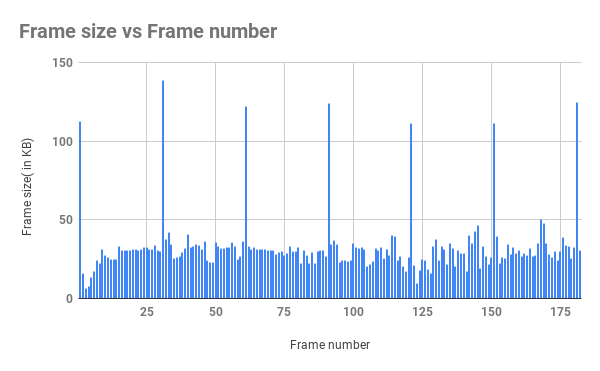
\includegraphics[width=1\textwidth]{/media/gunman/Data/thesis/ThesisLatex/data/images/FramesizevsFramenumber.png}
					\caption{Framesize of I and P frames}
					\label{fig:ex_4_9}
				\end{center}
				\vspace{-0.3in}
			\end{figure*} 
		%ffprobe lab.mp4 -show_frames
		Typically I frame to P frame is about ~4 times and we have one I for about ~30 P frames. This implies we save a lot on interface power if we can push the computation to near sensor.  
			
	d) Scaling with the resolution\newline
			Outputs:
			4k, 6k, 8k, 12k
		Discuss scalability of resolution for different stages. \newline
		Especially the scalability of cache, DRAM, CPU power. 
		

	e) Quality Tradeoff's with input resolution\newline
			Sharpening
			Reducing number of pyramid's
	f) High motion Vs low motion differences
	g) File IO power
	h) Breakdown in terms of type of Memory	used
	i) Breakdown in terns of type of Computation
	j) Breakdown in terms of IO bandwidth bottlenecks
	
	

2) Performance \newline
	a) Individual Stage Latency Characterization
	b) Breakdown of Optical Flow
		Individual Stage
		Time for each Pyramid Generation
	c) Breakdown of sharpening
	

 % Characterization and Bottlenecks(Research Questions)
%\chapter{Characterization}
\label{chap:Char}
The goal of the work is to characterize the energy and latency of end-to-end ODS camera  systems and propose optimizations. As the existing ODS camera systems are built from off the shelf camera devices and use the conventional stitching algorithms, they capture redundant data and perform redundant computations. The main challenge in ODS panorama generation is to understand the data flow across the system and to make decisions on data abstractions needed at different subcomponents to reduce the total system power and latency.

We classify our findings into two categories, i.e the reasons for high energy and high latency.
For high energy or power consumption, we divide into following three categories
\begin{itemize}
	\item Redundant Capture, and Computations
	\item High Data rates across interfaces
	\item Huge memory footprint
\end{itemize}
For high latency we analyze,
\begin{itemize}
	\item Effect of sequential execution on stage and sub-stage latencies.
\end{itemize}

\section{Measurement Methodology} % Energy and Latency Measurement 
Jetson has INA3221 monitors and I2C capabilities to read voltage, current and power for different rails on the SOC and IO. For evaluation we measure the absolute energy of the system and the difference between the idle and active state for individual stages of the pipeline. We also use NVIDIA Tegra stats command to check the clock frequencies of different components like CPU, GPU, Memory Controller for validation. 

The latency of the camera capture and ISP is defined by the framerate (i.e throughput), where for computation stages we measure the latencies in terms of CPU runtime of individual software components in the stitching pipeline. One of the critical components of stitching pipeline is optical flow which can take several seconds to compute each output frame on low power embedded CPU. Therefore for realistic estimation of optical flow for accelerator based design, we measure the power and latency of optical flow implementation on Zynq FPGA board. 

\section{Energy Characterization}
We first highlight the overall system energy profile. For the calculating the energy for frame in the above table, the camera capture is configured to 1920x1080 resolution at 30 fps, and the output resolution is 3k. We then explain about the key findings discussed in the introduction of this chapter. 
\subsubsection{Individual stage energy}

\begin{table}[h]
%		\\\specialrule{3pt}{0pt}{0pt}
	\begin{tabular}
		{!{\VRule[2pt]}c|!{\VRule[2pt]}c!{\VRule[2pt]}c!{\VRule[2pt]}c!{\VRule[2pt]}}
	Subsystem & Current(mA) & Voltage(mV) & Energy( mJ/frame) \\\specialrule{2pt}{0pt}{0pt}
	Sony IMX-274 (Camera) & 375.4 & 3336 & 41.7 \\\hdashline
	ISP+CODEC (TX2) & 102.7 & 19152 & 65.6 	\\\hdashline
	ARM-A57(Cap. + Stitch*) & 16.4 + 120* & 19144 & 10.5 + 36,736	\\\hdashline
	DRAM (Cap. + Stitch*)  & 260.4 + 105*  & 4792 & 41.6 + 1680 	\\\specialrule{2pt}{0pt}{0pt}
	\end{tabular} 
	\caption{Energy Characterization of Individual Stages}
\label{Tab:Energy_Char}
\end{table}

	Note*: As seen in the above table \ref{Tab:Energy_Char}, the stitching in software is highly expensive for CPU,and DRAM blocks, i.e the computation stage energy dominates the capture stage. CPU runtime to render each output frame of 3k is ~16 sec, which increases the both the energy and end-to-end latency. The other options include using GPU's, FPGA, ASIC's. Therefore, we approximate the energy and latency for FPGA based accelerator based on Xilinx's implementation of optical flow on Zynq board, discussed in chapter5.\newline

\subsubsection{Redundant Capture}
Natural images are redundant and but sensors are not smart to capture only the variations of the scene. Instead sensors capture and convert all the pixels for all the temporal frames. This leads to redundant conversion cycles by ADC's inside the sensor. It is therefore important to reuse the previous data to reduce the conversion cycles of the ADC to reduce the sensor power. 
\begin{figure}[h]
	\begin{center}
		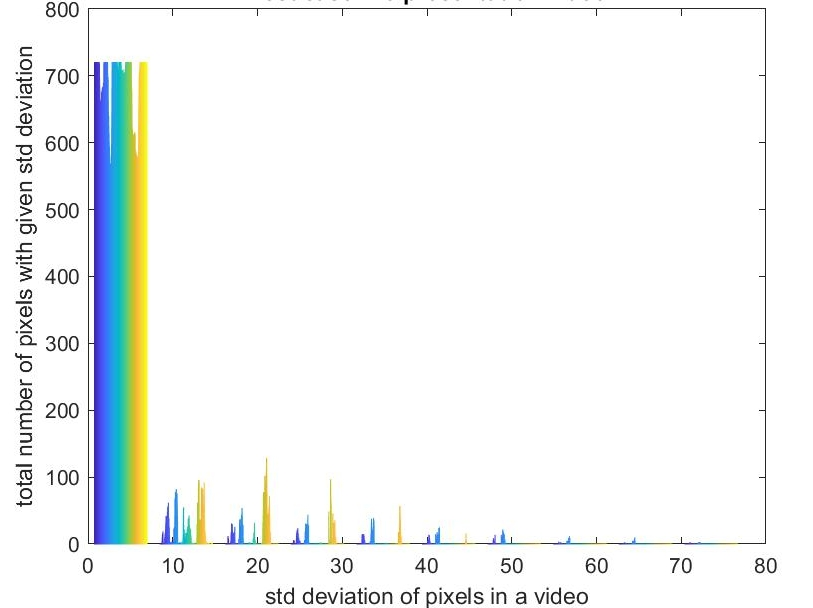
\includegraphics[width=1\textwidth]{data/images/Best_case_rio_presentation.jpg}
	\end{center}
	\caption{X axis shows the variations of pixels across 1000 consecutive frames, Y axis shows total number of pixels with a particular variation}	
	\label{fig:sensorRedundancy}
\end{figure} 

\subsubsection{High Data rates across interfaces}
As shown in the \ref{fig:pieCapPow}, the interfaces consume about one third of total power during capture. The high data rates lead lead to higher power consumption. But having compression near sensor and decompression near ISP will increase to high latency and may increase the sub-system power. A neat technique is to use the co-design of ISP with the interface encoding schemes. The ISP has Bayer statistics for different regions of the image. As the temporal frames are redundant, the Bayer statistics can be used for encoding CSI interface data efficiently. 

\begin{figure}[h]
	\begin{center}
		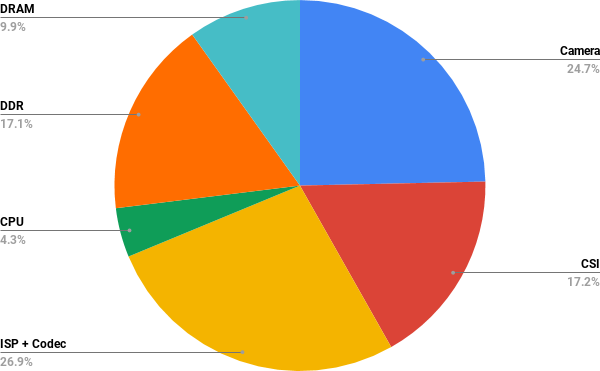
\includegraphics[width=1\textwidth]{data/images/chart.png}
	\end{center}
	\caption{Chart showing the distribution of power of different components during capture and storage.}	
	\label{fig:pieCapPow}
\end{figure} 

\subsubsection{Huge Memory Footprint}
The existing offloading based solutions have high memory footprint. One of the main reason being the inability to reuse the data generated by different subsystems. For example, during optical flow we load the current and previous image frames just to compute motion vector data. But this data is already available in ISP stage. Having data abstractions to reuse such data can reduce the memory requirement by up to 50 \%.


\subsubsection{Redundant Computations}
Similar to the sensor capture, the stitching algorithms perform lot of redundant memory access and computations. Even though only few pixels change between frames, the existing algorithms compute over the entire image for every frame. Building custom hardware with fine power gating can be used to reduce the activity of the computation units where the there is no motion across frames. 



\section{Latency Characterization}

\subsubsection{Individual Stage latency}


For camera system and ISP stages the stage latency is derived from throughput, i.e inverse of fps. The end to end latency is as given in NVIDIA camera API documentation, which is one frame latency for camera stage, and one for ISP stage. 

We measure the latency of computation in terms of CPU runtime. The optical flow, view synthesis and image sharpening stages take 98\% of total CPU runtime. The CPU  implementation takes 24 seconds for generating output at 6k resolution, of which optical flow generation consumes nearly 70 \% of runtime. We therefore focus on reducing the optical flow stage which dominates not just in terms of latency but also in power consumption. 


\subsubsection{Optical flow runtime breakdown}
The individual stages and the sub-stages of computation are sequential, leading to higher runtimes. By pipelining the different pyramid computation stages of optical flow, we can reduce the latency to 0.1 seconds from 16 seconds as shown in \ref{fig:OF_pyr_runtime}.

\begin{figure}[h]
	\begin{center}
		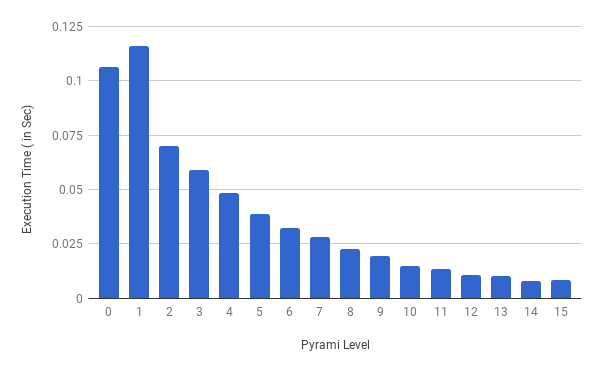
\includegraphics[width=1\textwidth]{data/images/pyramid_runtime.png}

	\end{center}
		\caption{X-axis shows the pyramid level and Y-axis shows the runtime for OF}
\label{fig:OF_pyr_runtime}
\end{figure} 

\section{Design Scalability}	

\subsubsection{Runtime scalability with the resolution}
As discussed in chapter 2 related work, the resolution required for next generation VR is at-least 16k and frame-rates greater than 120. For our evaluation, we assume that energy scales linear with frame-rate and focus our evaluation on scalability of increasing resolution. We can see in fig that even the runtime scales almost linearly with the resolution. Notice that optical flow dominates the total runtime, followed by view synthesis and image sharpening. We also measure the frequencies of CPU, DRAM controller with increasing resolution and observe [linear] dependency of clock frequency on the resolution.
\begin{figure}[h]
	\begin{center}
		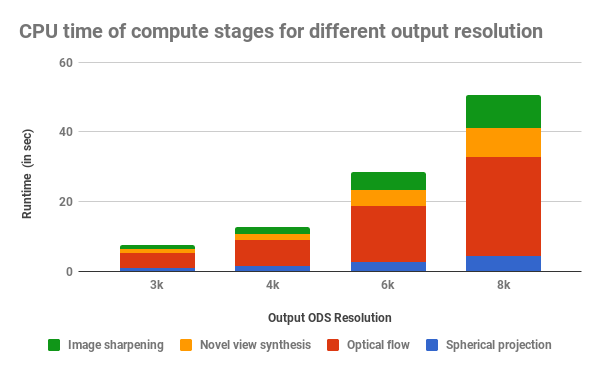
\includegraphics[width=1\textwidth]{data/images/ExecutionTimeComputeStages.png}
		\caption{CPU execution time of different compute stages. X axis has different sub-stages in optical flow and Y axis correspond to energy per frame.}
		\label{fig:ex_4_9}
	\end{center}
	\vspace{-0.3in}
\end{figure} 

The main takeaway is that the existing hardware and software scale linearly with the increasing resolution and framerate, which is bad considering the VR panorama requirements. We therefore propose directions to exploit the spatio-temporal redundancies within the frame and across the frames to reduce the data flow and computation. We propose rasterbuffer based design to decrease the chip resources, and use data abstractions at different hardware IP blocks to share data to reduce temporal redundancies(eg. motion vectors from ISP can be used by optical flow stage, thereby removing the necessity to store previous frames and recomputation of motion data at a later time. The same motion vectors can be used to encode spatial frame data to reduce redundant data transfer).
%What is the energy per each output pixel	
%What is energy per pixel when generating only one ODS view, and how does it compare when generating two views! If it is double then we have a problem to solve	
%[Check why sharpening is so costly!]

\subsubsection{Resource scalability with the resolution}
We measure the DRAM capacity and bandwidth needs as we increase the resolution as a parameter for resource scalability. Higher capacity indicates the need for better encoding schemes and high bandwidth can indicate the temporal redundancy in the data, thereby increasing the bandwidth requirement. For 3k, 4k, 6k and 8k output resolution.

Although we built a system where all the cameras are capturing at same resolution and framerate at a given time, we expect the future cameras make these decisions dynamically to save power. Therefore, we  measure the efficiency of capture and ISP processing at different modes of operation and measure the efficiency of capture and processing in power consumed per pixel at different modes.

% Figure 
\begin{figure*}
	\begin{center}
		\includegraphics[width=1\textwidth]{data/images/Power_Efficiency_of_Camera_ISP_Stages_in_different_configurations.png}
		\caption{Power Efficiency of Camera ISP Stages in different configurations}
		\label{fig:ex_4_9}
	\end{center}
	\vspace{-0.3in}
\end{figure*} 



\section{Different sensor configurations for energy efficiency and quality}
\subsubsection{Saving sensor power}
As the ODS consist of several cameras, it makes sense to reconfigure or turn cameras or off based on the application needs and the scene dynamics. If the camera is not moving and certain portions of the camera views are static, the cameras can be reconfigured dynamically to reduce framerate, resolution, or even turn them on and off as per the needs. We observed that the reconfiguration latency is one frame delay if there are no outstanding requests, and if there are pending camera requests, they will be served first before requesting the frame with new configuration. 
\subsubsection{Improving quality of images in low lighting}
The optical flow works well when the image is has high dynamic range. It is possible that some of the regions in the 360 degree view can be in low lightning, while other are in good lightning conditions. In such cases the stitching fails and can have severe artifacts. We can improve the dynamic range of the particular cameras in low lightning by reconfiguring the camera exposure time dynamically. But such approaches do not consider the end to end latency of the cameras and camera movements. To account for camera movements, IMU sensor data can be used to make the camera configuration decisions independent of CPU to accelerate the reconfiguration tasks. 

The figures \ref{fig:histLow} and  \ref{fig:histHigh} show the differences in low light capture with and without brightness correction.
	\begin{figure}[h]
	\begin{center}
		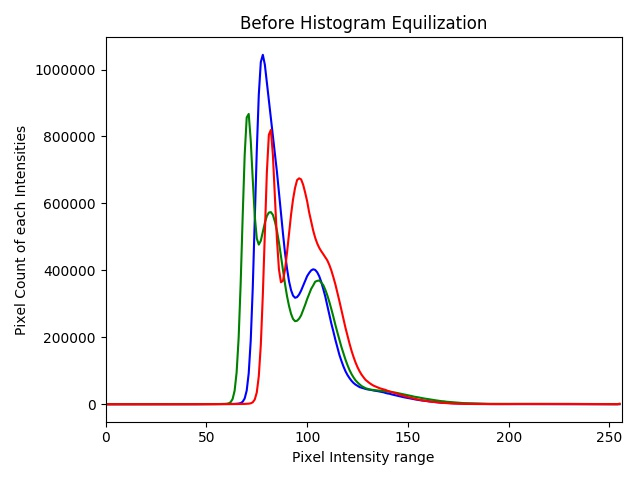
\includegraphics[width=0.8\textwidth]{data/images/Before_Histogram_equilization.jpg}
		\caption{Image intensity histogram for low lightning conditions}
		\label{fig:histLow}
	\end{center}
	\vspace{-0.3in}
\end{figure} 

\begin{figure}[h]
	\begin{center}
		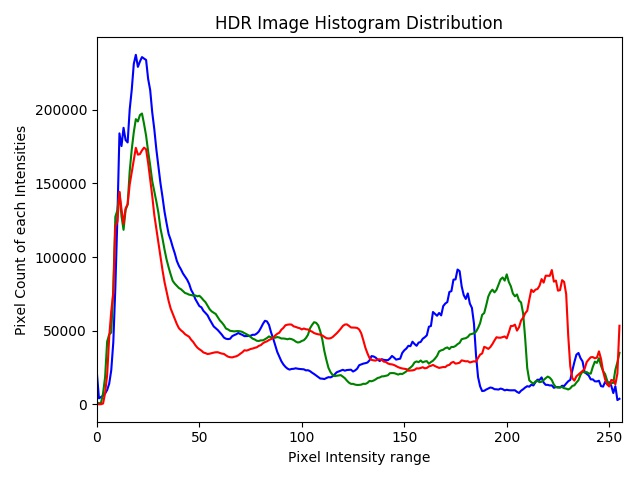
\includegraphics[width=0.8\textwidth]{data/images/Normal_Histogram_Distribution.jpeg}
		\caption{Image intensity histogram for good lightning conditions}
		\label{fig:histHigh}
	\end{center}
	\vspace{-0.3in}
\end{figure} 

 % Research Questions
\chapter{Proposed mechanisms} % for energy and performance savings

	Technique $\Rightarrow$ Benefits  \newline

1) Hardware software co-design: Re-using motion vectors generated by ISP stage to reduce the re-reference of previous image frames to calculate motion vectors for optical flow generation.\newline
(How to check if we need to compute everything with intensive vision algorithms or just use the precious results, what granularity to compute. Eg. Pyramids updating. Reactive to reconfiguration and powering on and off.)\newline
	a) Reduction of DRAM capacity requirement\newline
	b) Reduction of DRAM bandwidth requirement\newline
	c) Reducing end-to-end latency in generating dense optical flow \newline
The calculation of optical flow is the major bottleneck in terms of both memory usage and computation. The inputs for the optical flow include the current and previous camera frames of two adjacent cameras, their alpha channel and the previous optical flow. The need for temporal frames is to detect motion that is used of temporal flow regularization. Since the main memory is limited, the previous frames are usually stored in disk which increase the flow computation latency, and increase the DRAM capacity requirement and the bandwidth requirement. Instead of saving the temporal frames  for motion estimation, we can leverage the motion estimation hardware IP's that use optimal DRAM and completely remove the need to go through the disk. We model this by precomputing the motion vector and feeding with the image data. From our emulation, we found reusing the motion estimation reduces the disk utilization by \_\_ \%, the DRAM energy by \_\_ \%, improves the end-to-end latency by \_\_ \%. 
\newline

High Level Synthesis: HLS provide constructs to generate hardware that uses parallelism, pipelining, data reuse and streaming operations. On top of these we also need to do bitwidth optimization. 

2) Data driven execution: Use of motion vectors and previous optical flow to update the pyramids to make use intrinsic properties of foreground, background and motion in the scene.
	a) Reduces the number of computations 
		i) For building pyramids.
		ii) For calculating SAD(Sum of Absolute differences) during pyramid block matching.
	b) Reduces off-chip accesses
	c) Reduce end-to-end latency
\newline
Adaptive stitching pipeline *
Not all regions of the image have same level of difficulty for stitching. In an outdoor filming, most of the top portions are covered by sky, and ground is covered by road. So if those regions can be stitched with lesser effort(i.e reducing the number of iterations in stitching). Since we are going to do flow based stitching, the number of iterations is number of tiles size reductions in the flow based iterative stitching. 

3) Hardware Accelerator:
Streaming Architecture: Using raster buffers across the entire optical flow pipeline.(Number of rows is constrained by maximum motion in the scene)
a) Helpful for scalability to higher resolution
b) Reduces size of local SRAM and off-chip memory access.\newline

	\begin{tabular}{c|c|c|c}
	Power Rail & Diff. Current(mA) & Voltage(mV) & Energy ( mJ/frame) \\
	ISP+CODEC & 102.7 & 19152 & 65.6 \\
	CPU & 16.4 & 19144 & 10.5 \\
	DDR & 260.4 & 4792 & 41.6 \\
	Camera & 375.4 & 3336 & 41.7 \\
	CPU & [] & [] & [] \\
	Accelerator[Zynq] & [] & [] & [] \\
\end{tabular} \newline 


Case for low power 360 capture. Real time Stitching 30fps >4k resolution with low power. 
Latency of GPU, CPU makes them unusable for vision tasks in AR, VR.
Case for algorithm software Co-Design for a line buffer based streaming architecture. \newline

GPU Based Acceleration.
NVIDIA Tesla: A unified graphics and computing architecture. E. Lindholm, J.Nickolls, S. Oberman, and J. Montrym. IEEE HotChips 2008
The paper gives an introduction to graphics and parallel computing capabilities of Nvidia Tesla. The organization of GPU from hardware and software aspects is explained in detail. A GPU, in general, will have one or more streaming multi-processors(SMT). The SMT in Tesla consist of 8 Streaming Processor cores. The serial part of the code is implemented in CPU, whereas the Graphics and parallel computing are done in SP cores of GPU. The SM is hardware multi-threaded. It creates and executes a group of 32 threads which are of the same type of operation. They are called warps. GPU has three types of memories local global and shared. Local memory is allocated each thread and is physically located in DRAM. Shared memory is located near SMP, and used by cooperative thread arrays( thread blocks). The global memory is in DRAM and is used by sequential grids( set of blocks) to communicate large data sets. The paper also talks about CUDA programming model. In CUDA the parallelizable kernels are implemented in terms of grids and blocks and given to GPU.

1) Energy Characterization of end-to-end pipeline\newline
Camera, ISP, Computation \newline
Split of energy in computation \newline
\newline
2) Runtime Characterization \newline
a) End-to-end pipeline\newline
b) Split in computation execution\newline
\newline
3) Performing motion estimation prior to computation stage\newline
a) Savings in DRAM capacity, bandwidth(Normalized) \newline
b) Savings in DRAM Bandwidth\newline
c) Savings in overall energy\newline
d) End-to-end latency reduction\newline
\newline
4) Optimizing of computation in pyramids \newline
a) The execution time split for creation of pyramid, finding optical flow of pyramid, refining/updating the pyramids, upscaling the pyramid. \newline
98 percent is to generate optical flow(dense pixel correspondence). But only 20-30 percent actually needs to be recomputed.\newline
Main optical flow method time is 0.560256
Total time for entire optical flow is 0.584954   
 

 5) Sense the environment in gray scale and perform color mapping later? How much are you saving? 
 
 6) Egocentric motion 

7) RAM-less architecture
RAM-less architecture is possible for panoramic stitching as we plan to process data and instantly stream the processed row data from one stage to another, instead of performing computation on full image.  We need to make the computation stages generic so that it can be extended to other applications with the use of same hardware resources. We also need to work on how to program the computing units and coordinate communication between computing stages. When we generalize streaming architectures we may create idle resources in computation stages for which fine grain power gating and clock gating techniques can be used to save power from the gates that are idle. 

There can be streaming applications where the DRAM might be necessary, in such situations our architecture should be able to support the DRAM with ease. Therefore our architecture need to be flexible to include DRAM if required.

Poster data \newline
Recent advances in image sensor technology and lens designs have led to the emergence of
portable spherical panorama systems, such as the Samsung Gear 360, capturing information to
process into 360ºx180º images and videos. However, real-time, energy-efficient generation of
high-resolution spherical panoramas remains a substantial challenge, as standard
computational architectures are incapable of efficiently processing large amounts of data.
Because energy consumption generates heat, creating imaging artifacts, e.g., lens warping,
spherical panorama systems are constrained by a tight energy budget. This has led commercial
implementations to offloading-based designs, in which stitching is done on the smartphone, and
not in real-time. These implementations are incapable of scaling to large resolutions, due to
limited and energy-expensive network bandwidth. Our proposed research will create designs
that efficiently scale to ultra-high resolutions into the future, based around streaming spherical
panorama architectures that do not rely on DRAM, memory storage, or other expensive I/O
during processing. We estimate that this will create a sub-watt architecture to generate and
transmit 4K 360º video under 1 watt on the portable spherical capture device. \newline

We propose two key research goals: (i) Establish an efficient RAM-less streaming
architecture to direct fisheye sensor data into equirectangular output; and (ii) Study the effects
of early in-sensor compression to reduce the transmission of data across sensor interfaces.  \newline

\section{Stereaming feature detection and Correspondence}

We propose an architecture for feature detection and correspondence that makes effective use of spatial locality towards pixel buffers and divide-and- conquer strategies, allowing an independence from random-access memory. We expect that features detection and correspondence operations can be derived from standard corner-based algorithms, but propose to study novel hardware designs for area-efficiency and energy-efficiency. \newline

To further reduce the energy consumption of the system architecture proposed in Thrust 1, we target the image sensor physical interface as a bottleneck to energy efficiency. As temperature requirements force a substantial distance between image sensors and processing units, sensor data transactions are notoriously energy-expensive. At full input resolution of 15 MP at 30 frames per second, using a typical Low-Voltage Differential Signaling (LVDS) physical interface consumes 2W to satisfy the \&gt;3 Gbps bandwidth, e.g., [8]. This is prohibitively high, and the Gear 360 typically is constrained to capture video at one half of this available resolution, while still consuming multiple watts of average power consumption. We explore the use of in-sensor compression to assist in an energy reduction, as compared in Table 1. Existing hardware solutions for JPEG and MPEG compression are plentiful and sufficient, dropping data \newline
bitrates by substantial compression ratios (e.g., 8:1, 23:1, 46:1, etc.) and some image sensors integrate real-time JPEG encoders into their package [9]. As shown in Table 1, this can have dramatic savings on interface power consumption. Using this as our basis, Thrust 2 proposes system-oriented research for placement and utilization of compression hardware close to the sensor. Thrust 2 aims to approach research objectives of (i) processing on the compressed data, i.e., without decompression; and (ii) region-based compression quality.\newline
----------------------------------------------------


\section{High and Low Resolution combination}
What are the regions of the image frame that are needed in high resolution in order to generate a high resolution output ODS video. 
\begin{figure*}
	\begin{center}
		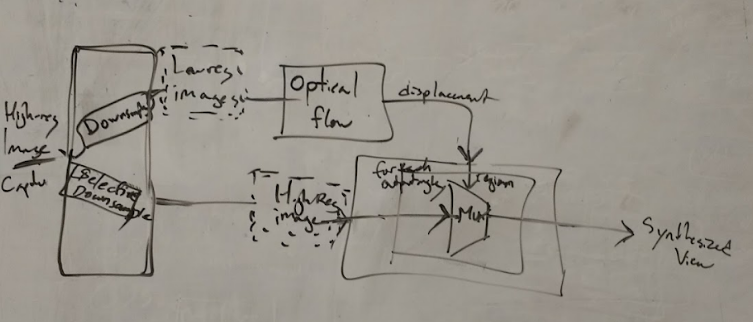
\includegraphics[width=1\textwidth]{/media/gunman/Data/thesis/ThesisLatex/data/images/HIgh_low_res_architecture.png}
		\caption{X-axis shows the pyramid level and Y-axis the runtime tile search and propagate.}
		\label{fig:ex_4_9}
	\end{center}
	\vspace{-0.3in}
\end{figure*} 








 % Proposed Mechanisms
\chapter{Discussion}
Summarizing the proposed optimizations and future directions.
DRAM-less
Stacked Image Sensors
ADC readout power, Rolling vs global shutter
Abstractions for hardware software co-design
a) How to find out which data to sense, send without the intervention of computationally intensive vision algorithms.
b) How to detect them early in the vision pipeline
c) Data Driven 



	

 % Discussions
\chapter{Conclusion}
Real world content generation for VR is an emerging research problem. VR content needs to capture 360 degree views and 3D immersive experiences. The existing 360 camera devices have portable camera rigs that capture and offload the expensive computation to cloud, or powerful desktops. This limits the scalability of stitching operation  and increases the end-to-end latency. But performing capture and generating the VR panorama on the same device is computationally expensive. 	Our work focuses on characterizing the energy and latency of end-to-end Omni-directional(OD) Camera  systems. Through the rigorous process of building prototype and evaluating the power and latency of the system, we found that by reusing and reducing the data across different stages of pipeline, we can optimize the system for power. By pipelining and parallelizing the compute in hardware, we can reduce the latency. The end-to-end system latency with proposed design is in the order of 100ms and the system power in the order of 3-5 Watts.
%Although commercial solutions exist, the dataflow is broken resulting to long latencies and high computation power.

% The workflow consist of camera that captures the multiple views and offload the computing to desktop or cloud for stitching the video. These solutions needs several 1000's of CPU's if not multiple GPU's consuming consuming upto 1 kilo Watt power. Cloud based solutions will have high latency making it challenging for real-time streaming. We envision that capturing and rendering near camera helps improving the end-to-end latency and reduce the power by close integration of the capture and rendering system. 

 % Conclusion and Future Work
%-----------------------back matter
{\singlespace
% Making the references a "part" rather than a chapter gets it indented at
% level -1 according to the chart: top of page 4 of the document at
% ftp://tug.ctan.org/pub/tex-archive/macros/latex/contrib/tocloft/tocloft.pdf
\addcontentsline{toc}{part}{REFERENCES}
\bibliographystyle{asudis}
\bibliography{dis}}
\renewcommand{\chaptername}{APPENDIX}
\addtocontents{toc}{APPENDIX \par}
\appendix
\chapter{Raw Data}


Data Flow \newline
Block Diagram
- With different stages.
- With Data Inputs and Data Outputs of each stage. (Zoom in Diagram)

\begin{figure*}
	\begin{center}
		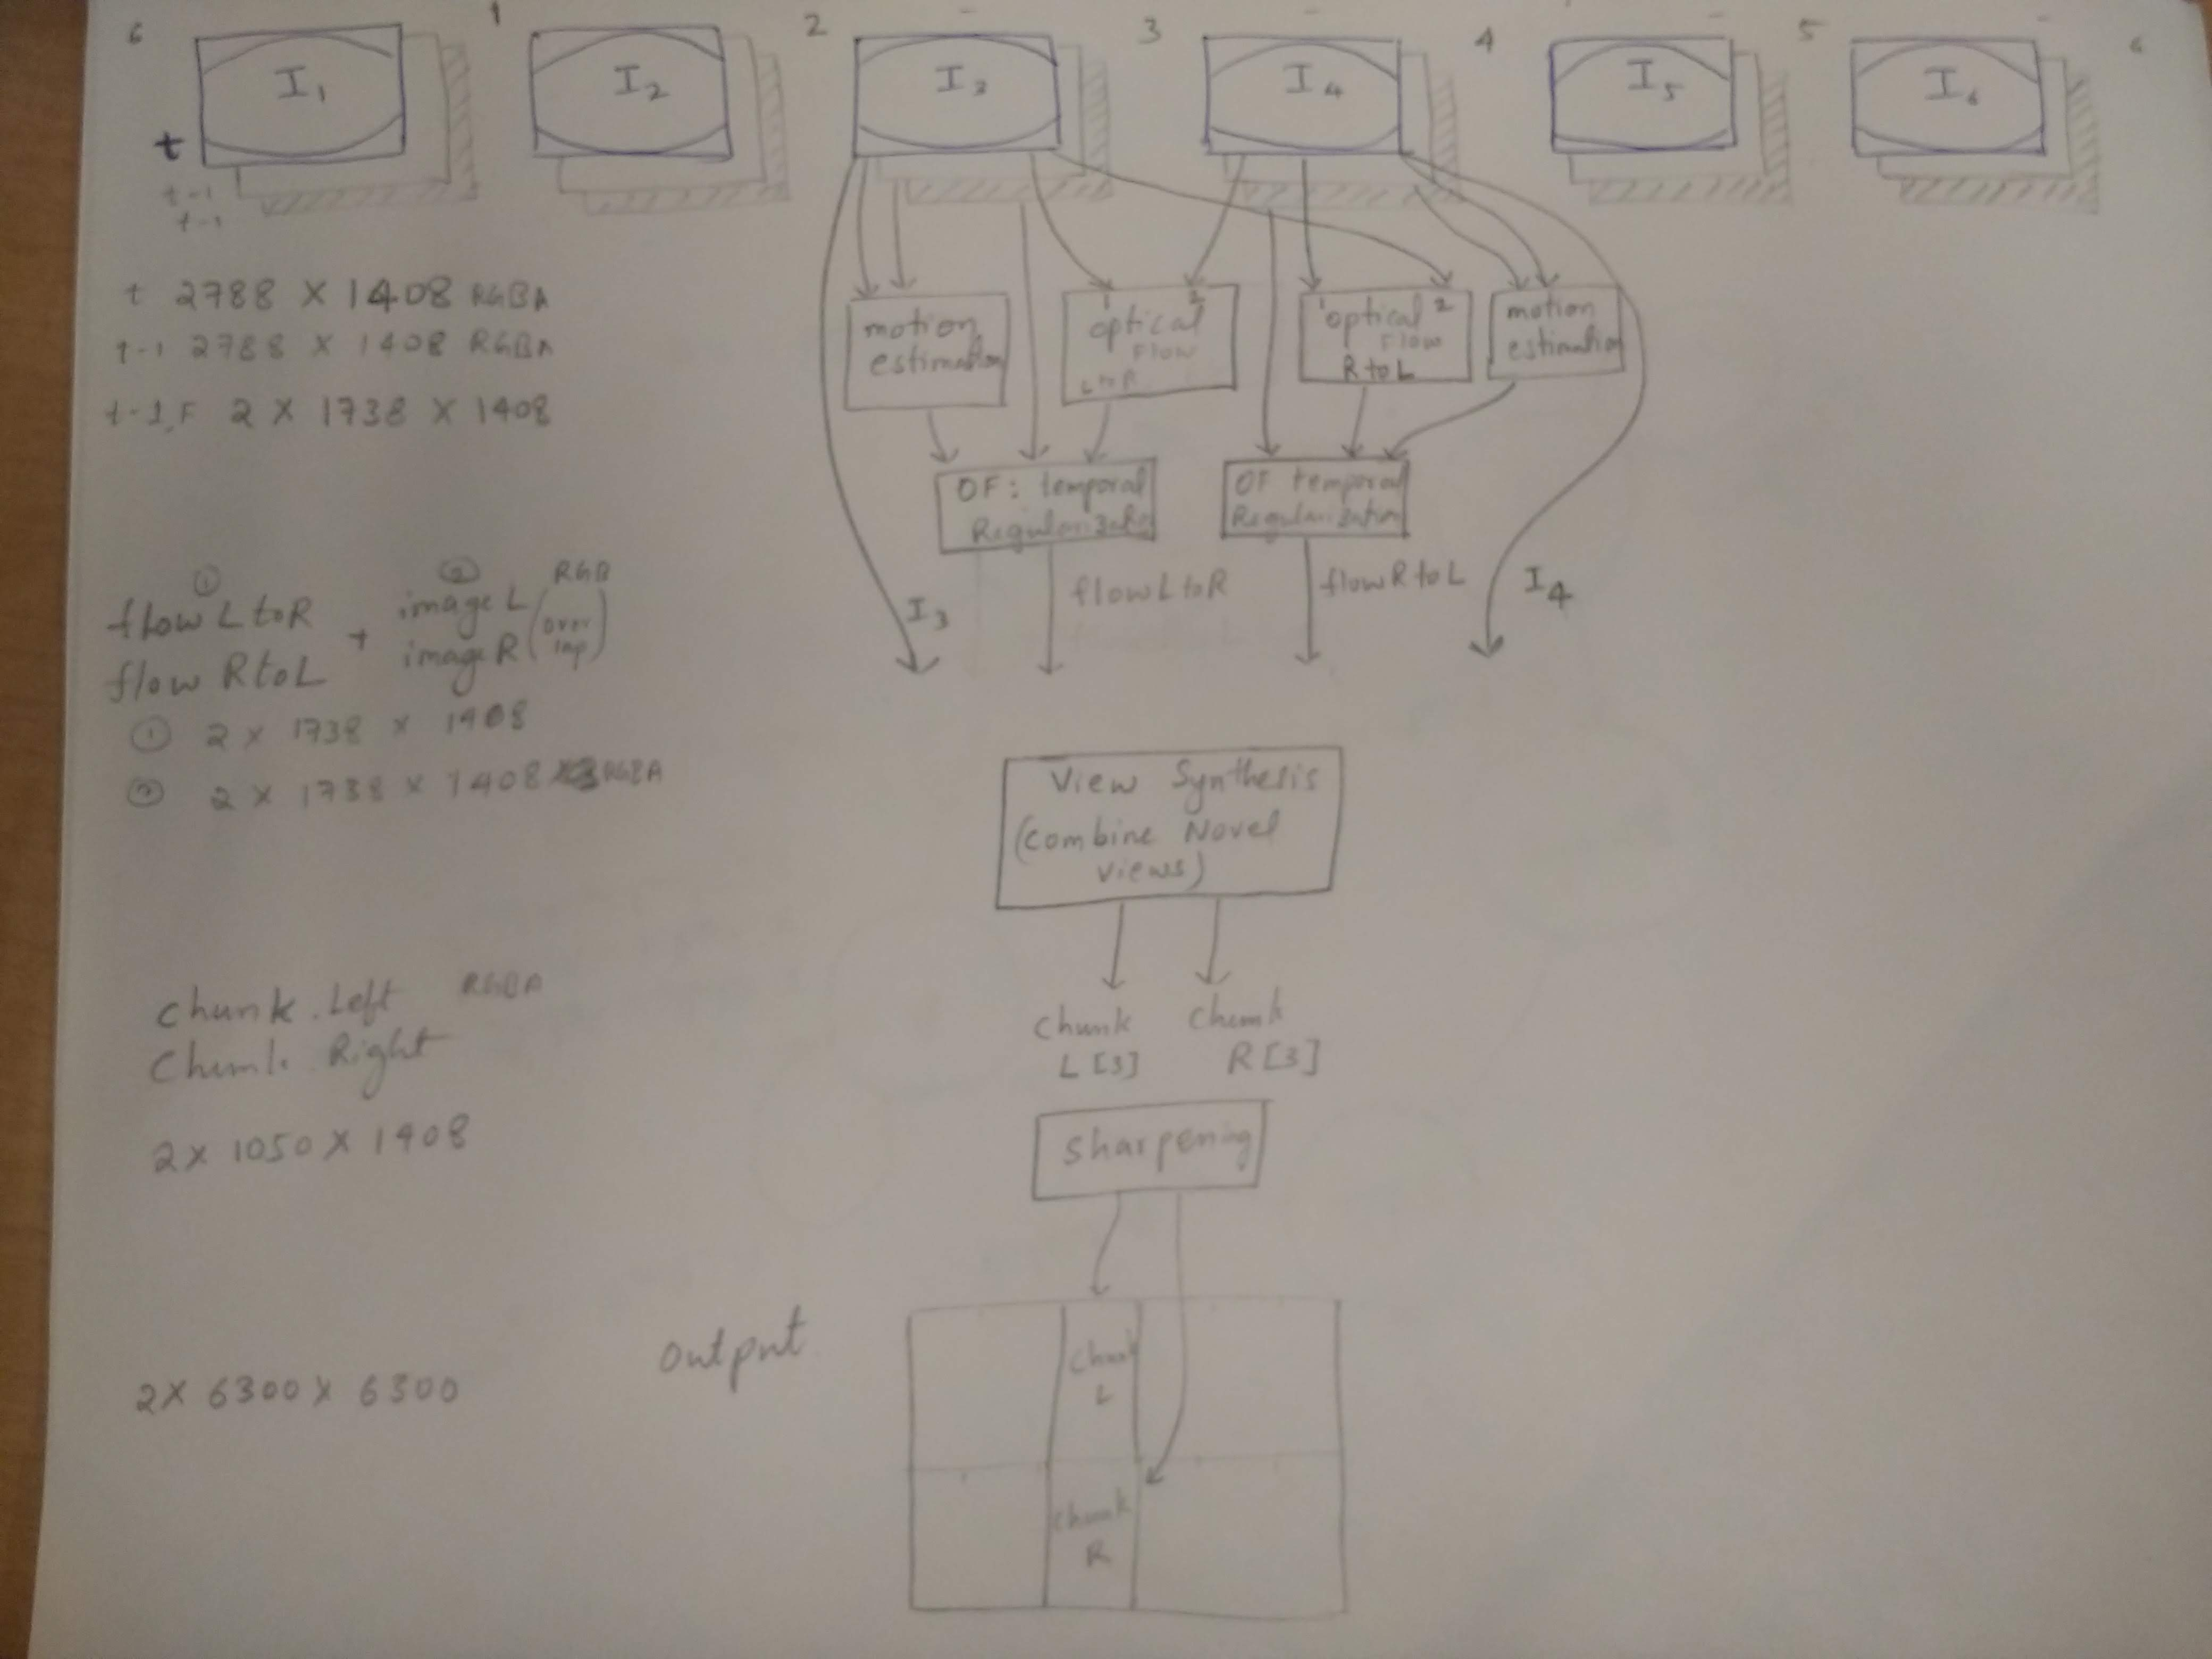
\includegraphics[width=1\textwidth]{/media/gunman/Data/thesis/ThesisLatex/data/images/ODS_Input_Output.jpg}
		\caption{X-axis shows the pyramid level and Y-axis the runtime tile search and propagate.}
		\label{ODS_Input_Output}
	\end{center}
	\vspace{-0.3in}
\end{figure*} 

The fisheye camera images.

\begin{figure*}
	\begin{center}
		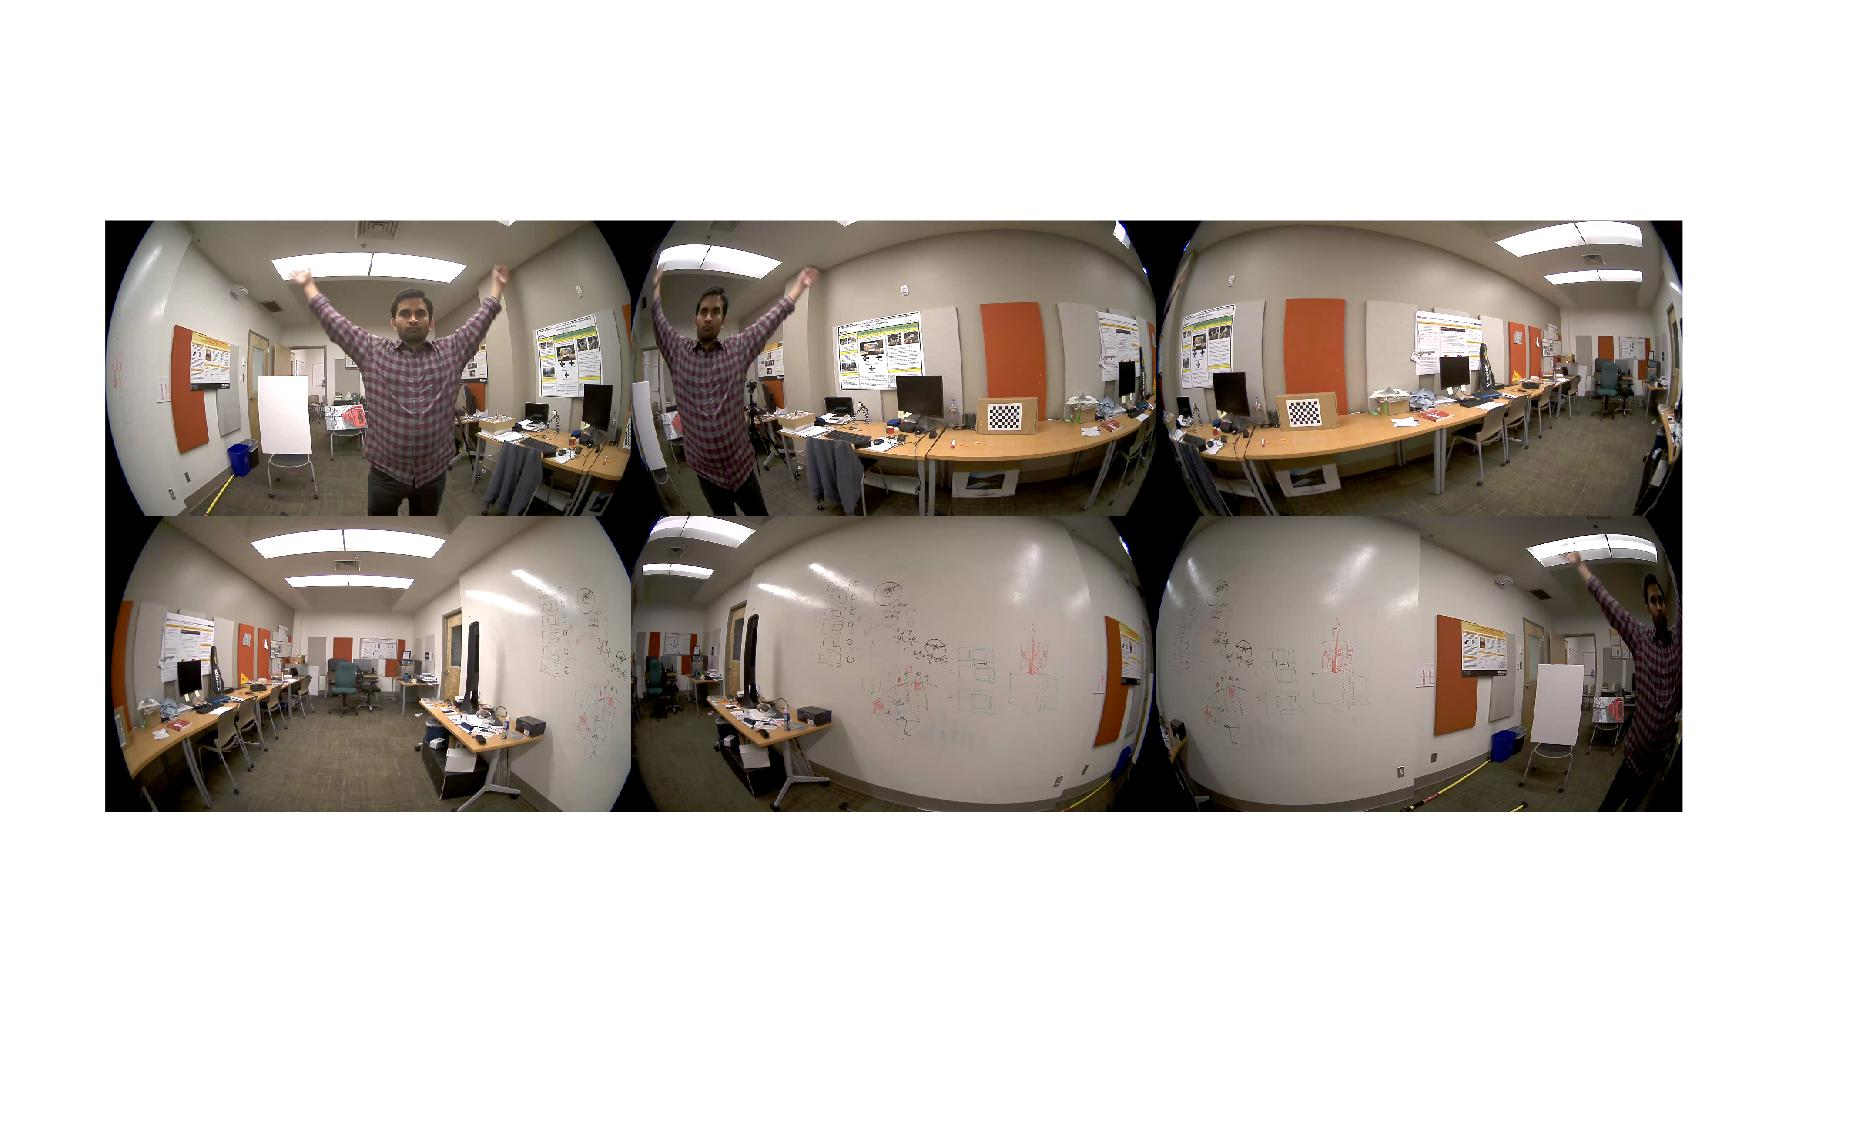
\includegraphics[width=1.1\textwidth]{/media/gunman/Data/thesis/ThesisLatex/data/images/fisheye_all6.jpg}
		\caption{Six fisheye images as captured by the IMX274 using Jetson TX2 board.}
		\label{ODS_Input_Output}
	\end{center}
	\vspace{-0.3in}
\end{figure*} 

The Equirectangular projection.

\begin{figure*}
	\begin{center}
		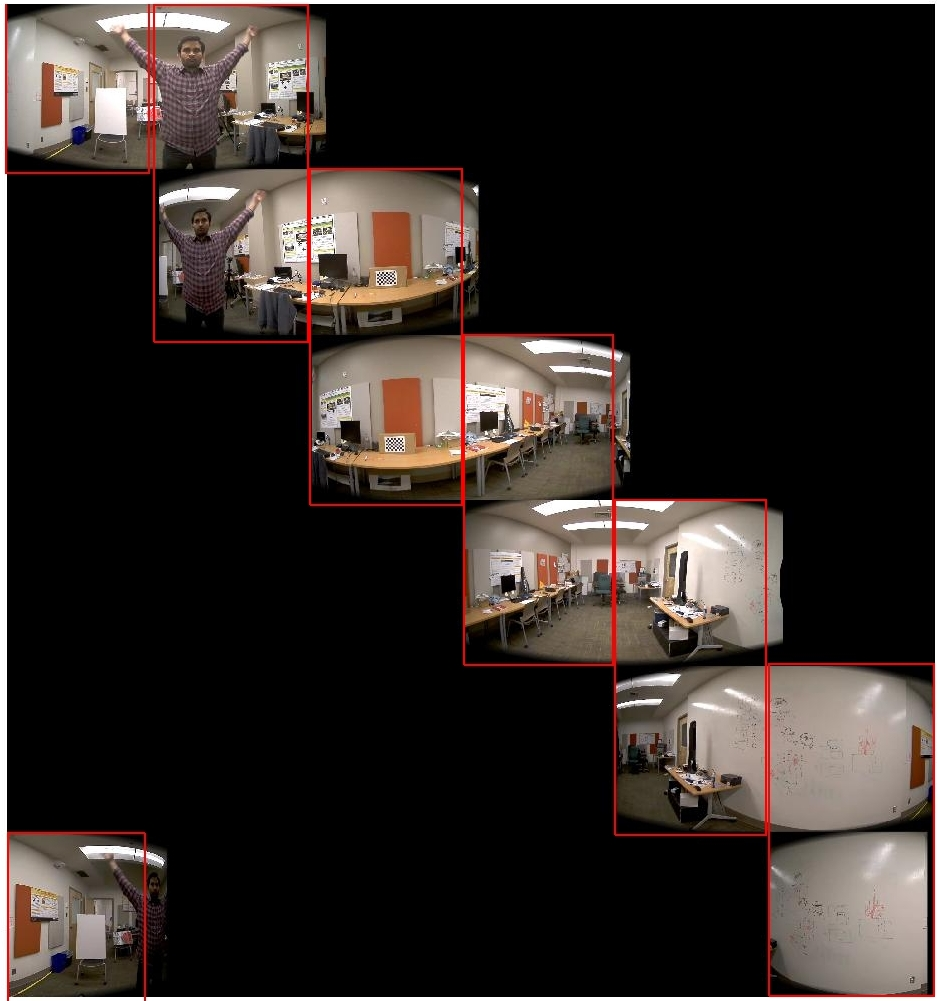
\includegraphics[width=1.5\textwidth]{/media/gunman/Data/thesis/ThesisLatex/data/images/EqRect_offset_fov_viz_loop v3.jpg}
%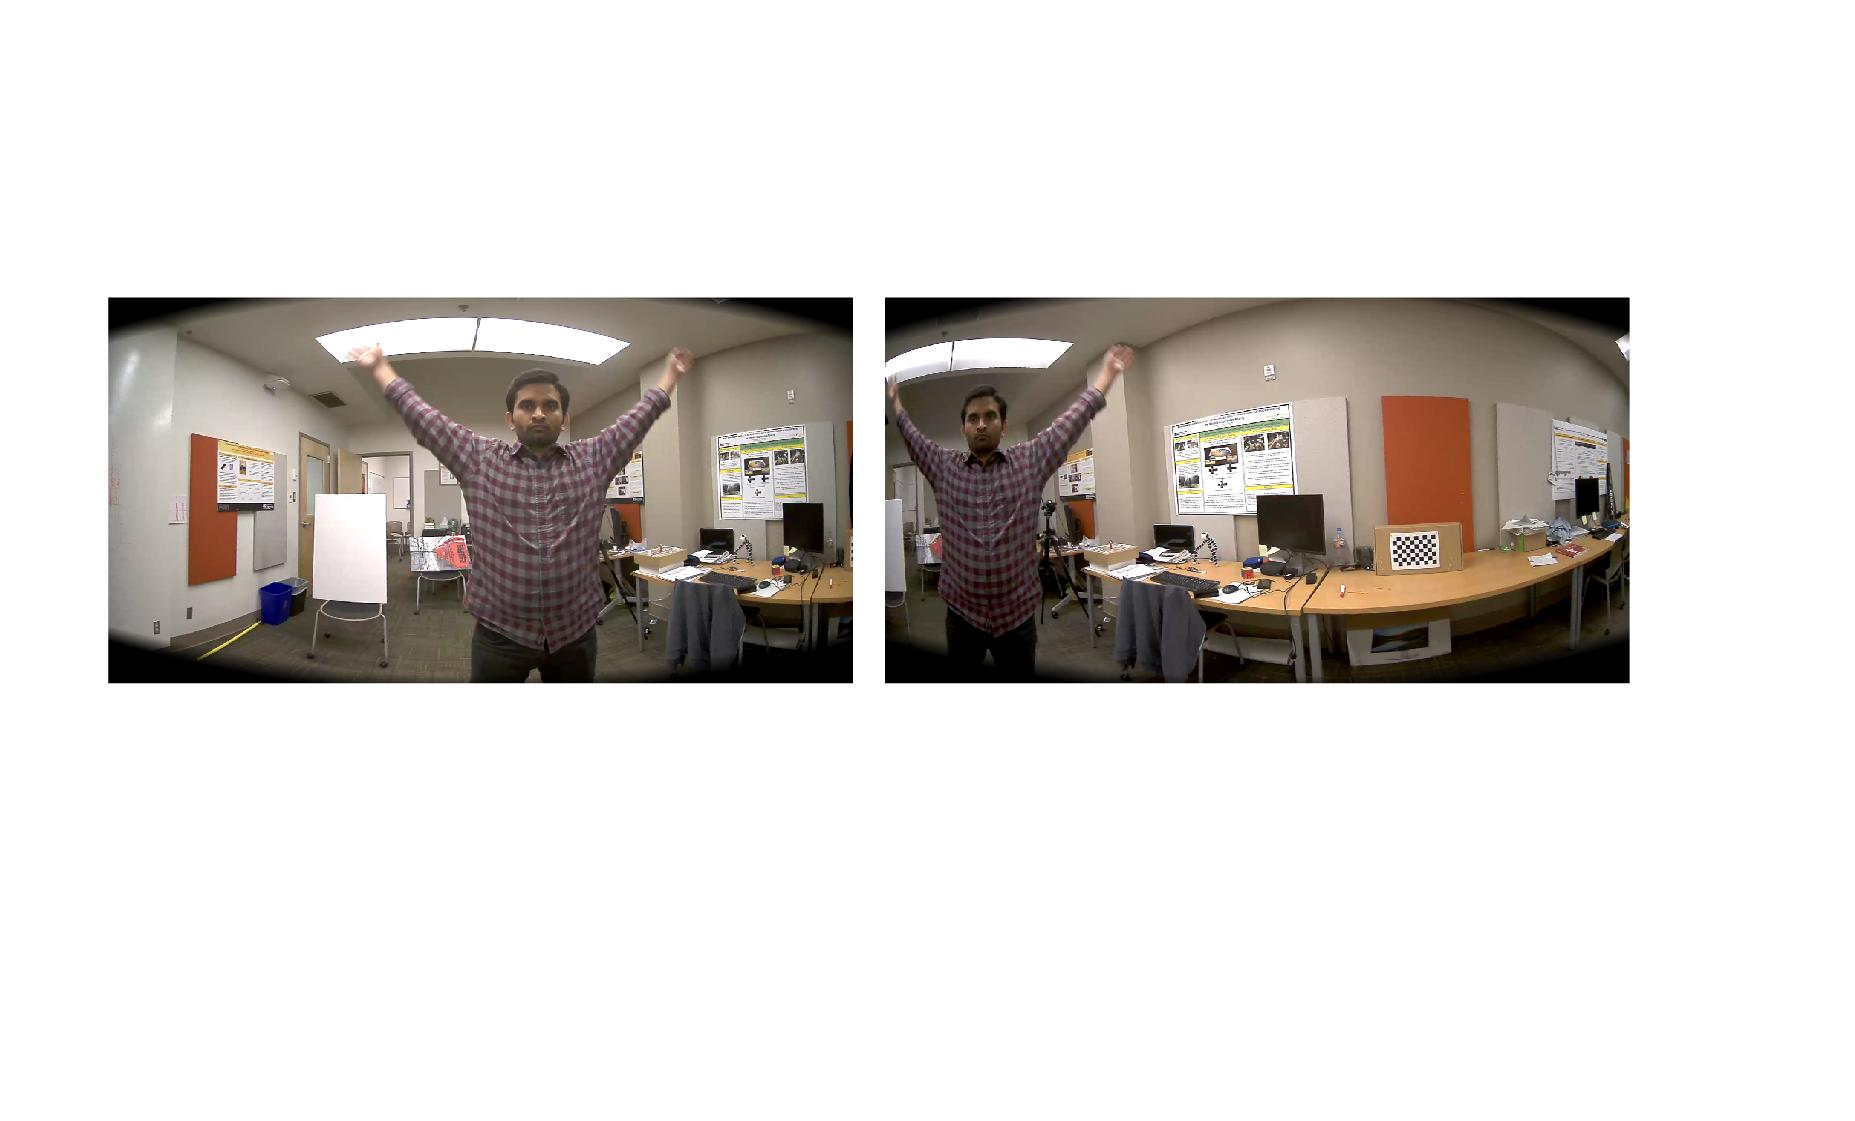
\includegraphics[width=1.1\textwidth]{/media/gunman/Data/thesis/ThesisLatex/data/images/EqRect_2_adj_images.jpg}
		\caption{Equirectangular Projection of first and second camera frames}
		\label{ODS_Input_Ouput}
	\end{center}
	\vspace{-0.3in}
\end{figure*} 

The overlapping left and right images.
\begin{figure*}
	\begin{center}
		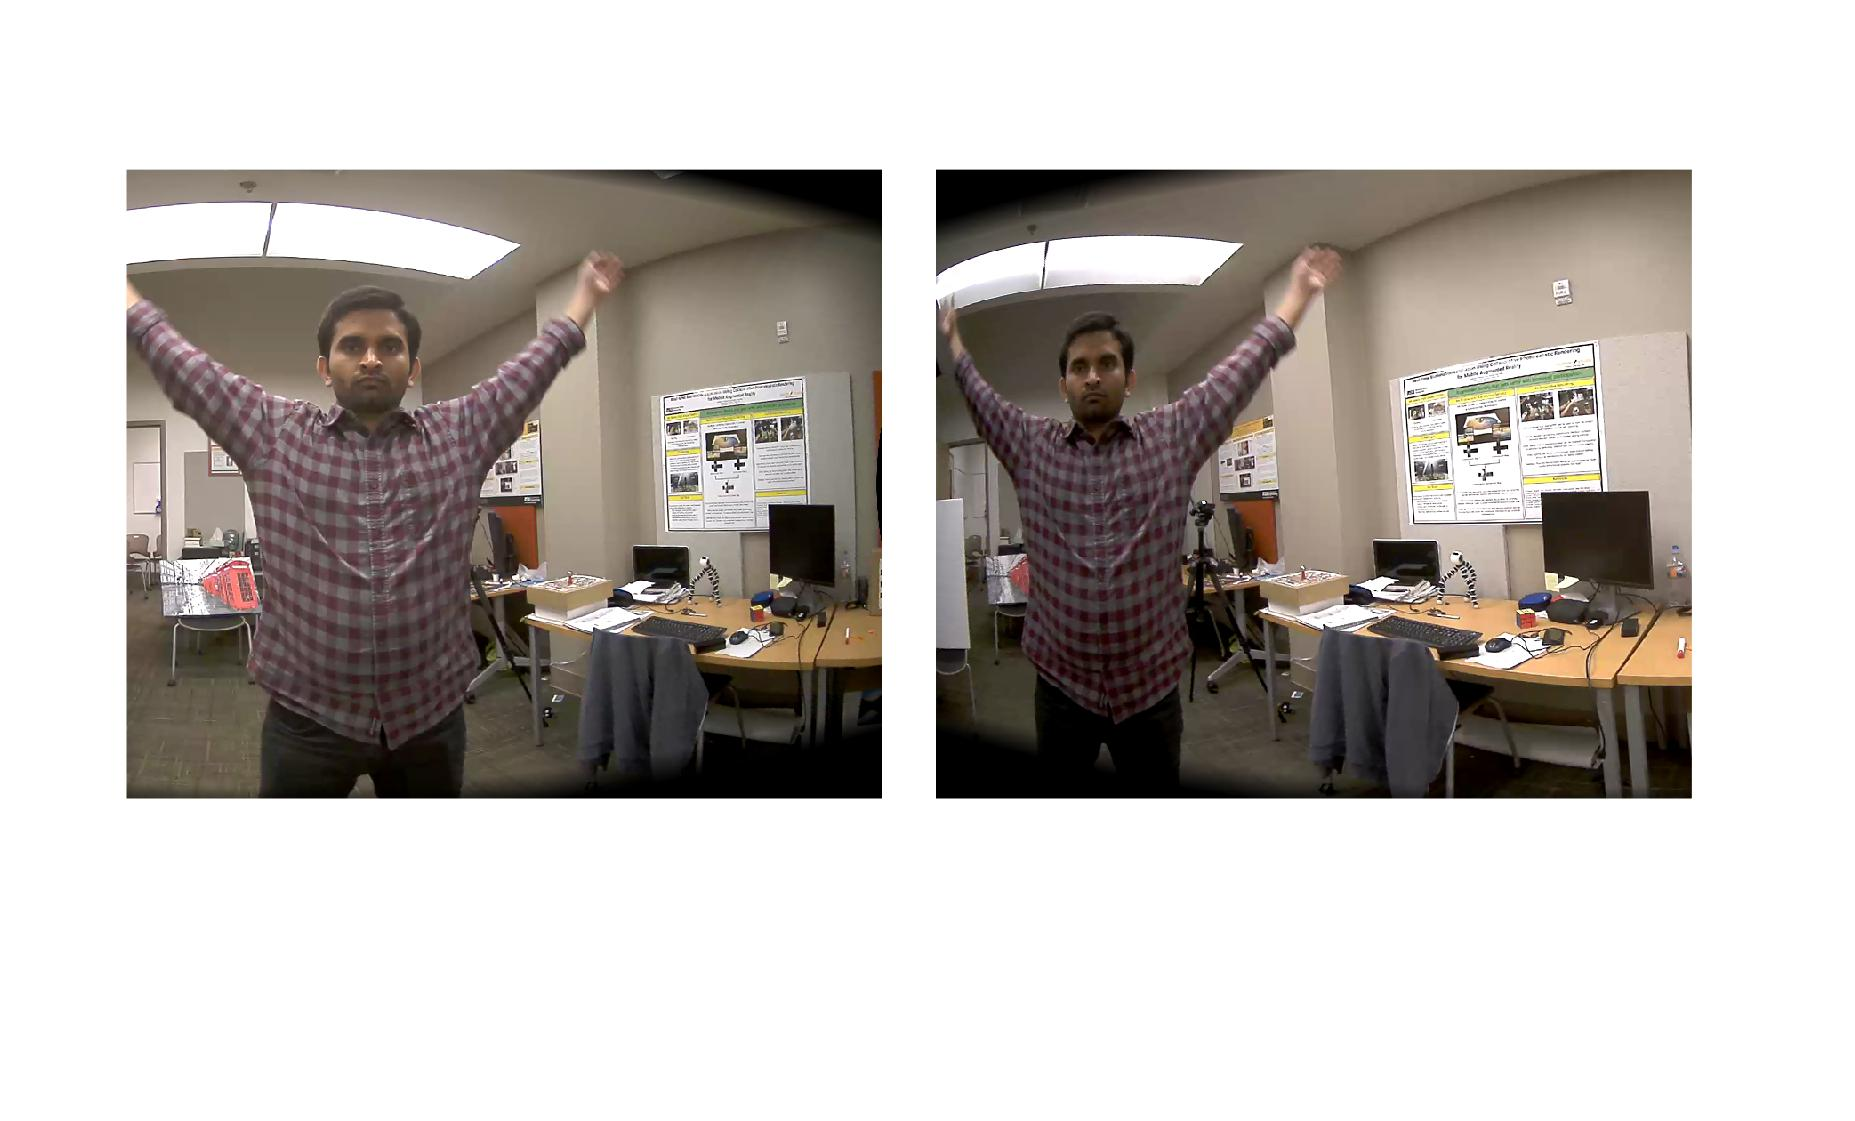
\includegraphics[width=1.1\textwidth]{/media/gunman/Data/thesis/ThesisLatex/data/images/OF_inp_overlap_region_of_adj_cam.jpg}
		\caption{Optical flow inputs: Overlapping regions of adjacent camera images. Equirectangular Projection of first and second camera frames}
		\label{ODS_Input_Ouput}
	\end{center}
	\vspace{-0.3in}
\end{figure*} 


\begin{figure*}
	\begin{center}
		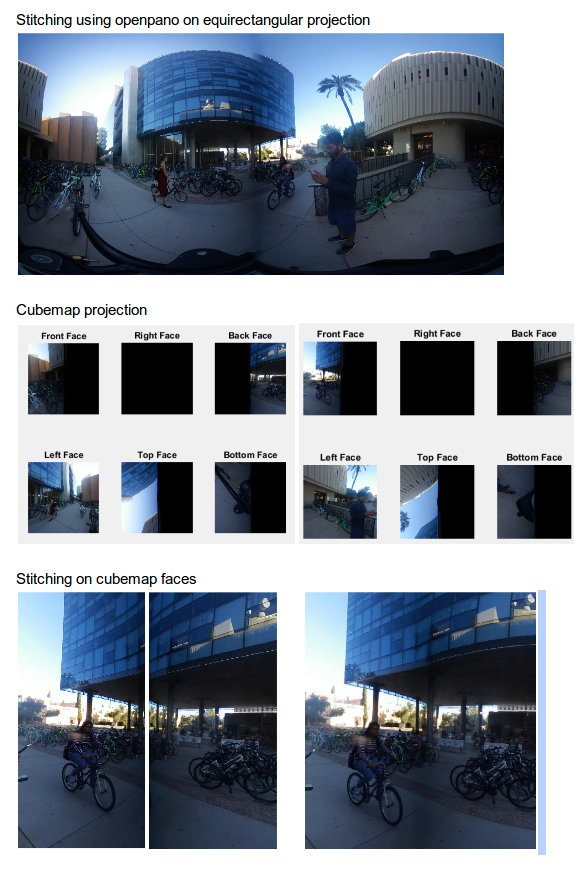
\includegraphics[width=1\textwidth]{/media/gunman/Data/thesis/ThesisLatex/data/images/CubeMapBasedStitching.png}
		\caption{Cubemap based Stitching, Path : /media/gunman/Data/fall-2017/research/mono360/equi2cubic}
		\label{ODS_Input_Output}
	\end{center}
	\vspace{-0.3in}
\end{figure*} 

Maximum Function For Extreme low power applications:
Since the alignment techniques is not the final algorithm I may be going ahead with, I want to start with something even simpler, i.e a maximum function. We can imagine the core computation block as a black box, that can be changes as per the needs of the application. This becomes an interesting use case as the final camera could have multiple such black boxes which can be turned on and off based on application demand. For eg. If the camera is being used for CNNs, maximum function might be good enough. If it’s going to be used for scene capture, then we can turn on an efficient stitching core instead of maximum function.






\chapter{Making of the camera rig}

Camera Calibration Process
OCamCalib
%https://www.mathworks.com/help/vision/ug/fisheye-calibration-basics.html?s_tid=gn_loc_drop

%https://medium.com/@kennethjiang/calibrate-fisheye-lens-using-opencv-333b05afa0b0
%https://medium.com/@kennethjiang/calibrate-fisheye-lens-using-opencv-333b05afa0b0



\chapter{Systems Architecture Survey}
Heteregeneous Systems
Memory Access scheduling has been very critical since the single core processor. [5] Rixner et. al. introduced the scheduling of DRAM operations out of order, to optimize memory system performance. They reordered the memory references to exploit row buffer locality. But the major drawback of this kind of memory schedulers was they optimized for throughput rather than for the overall performance of different application threads in the system. This became more evident with the chip multiprocessors(CMP). Mutlu and Moscibroda proposed a Stall Time Fair Memory(STFM) Access Scheduling[4] to overcome these issues. STFM provides quality of service(QoS) to all the threads by measuring the slowdown of threads. The results show that slowdown related to thread level interference is significantly reduced and also, it improved average system throughput.\newline
In the last few years, hardware accelerators have dominated the SoC from mobile to High-performance computing. The modern mobile SoC’s[7, 8]  are heterogeneous architectures that integrate CPU with hardware accelerators like  GPU, image processor, audio processor. On the other hand, High-performance Computing clusters are now being accessible through cloud services like amazon web services[9] and others.  Heterogeneous System Architecture(HSA) [11] is being developed by multiple companies to integrate CPU and GPU unified virtual memory.  As a step further Unified memory is currently introduced in Nvidia CUDA 6. All of this motivates to further study on application interference, meeting QoS targets for close integration of CPUs and GPUs.\newline
The heterogeneous systems are currently being optimized to have same off-chip memory and even share ldast level Cache to reduce area, remove memory copy overheads and for tighter integration between CPU and Hardware Accelerators(HWA).  The sharing of resources lead to interference in memory scheduling if not prioritized efficiently. Since the heterogeneous systems are required to provide support to multiple application, QoS of each application becomes very critical. Several works have proposed in this area[1,2,3,12]. Staged memory scheduling [1] proposes a new approach to improve system performance and fairness, especially in integrated CPU-GPU systems. Although it provides fairness, it doesn’t take care of strict QoS requirements by applications. Jeong et al.[12] prioritize applications when the HWA’s are unable to meet the application deadlines. This mechanism doesn’t help resolve the QoR issues completely as the applications don't meet the deadline when they are prioritized very late.  Dash, Squash [2,3] propose ideas to overcome this. Their first idea, Distributed Priority, prioritize the HWA when they are distant from the deadline, thereby removing the risk of missing the deadline.  Their second idea is application aware scheduling for CPU’s.  This is based on the observation that memory intensive CPU applications are not affected when HWA’s are given priority over them. The third idea is to prioritize HWA’s with a short deadline with the highest priority when they are close to the deadline.\newline
The DASH and SQUASH schemes mainly focus on applications where there are multiple kinds of HWA’s, and there is contention for memory resources. This kind of systems is common in mobile systems. But there is another breed of heterogeneous systems which is dominated by GPU’s and CPU’s, mainly used in high-performance computing(HPC). The ideas given in Dash and SQUASH cannot be directly applied to HPC systems. Through this project, I plan to study the heterogeneous systems dominated by GPU’s. The characterization studies by [13, 14] make observations related to CPU-GPU systems.  [14] evaluates the performance seen with coarse grain and fine grain synchronization. They test two types of memory configurations, i.e separate L3 cache vs shared L3 cache. [13] concludes that shared LLC will provide better caching for heterogeneous processors compared to discrete GPU systems. So my project will focus on evaluating the performance bottlenecks and the meeting the QoS requirements for CPU-GPU based heterogeneous systems where Last Level cache is shared.\newline

References:


Experience With FPGA Vs NVIDIA Jetson: \newline
Last week’s target is to complete the Alexnet CNN layer C1 to C5 operations using DRAM based FPGA implementation. Since the run time of the tools is in the order of hours and even days(for place and route step), I planned my work as follows. I have divided my work into two parts. First one is to take simple accelerator design(AXI, AXI-lite based simple accelerator + Microblaze ) and perform  IP integration, generating the drivers files. Xilinx SDK will then be used to write c program using driver API’s to transfer data between microBlaze and AXI-based memory-mapped I/O interface of the simple accelerator.  The second task is to take the actual design C1-C5 layers of Alexnet through same steps. The first task is successful. I used Xilinx SDK tools to write simple c-codes to transfer data between microblaze and accelerator. I used axi-lite interface of the accelerator to send and receive the data using microblaze. 

The second task is to take the actual design through the same design flow and use drivers API’s to do data transfer. Before doing that I needed to rewrite the c++ code to make sure that all the data required by CNN accelerator can be received by single AXI interface(burst mode). I changed it so that accelerator will get the start pointer of array, and control signals(start, stop)  through axi-lite interface and then the accelerator will make memory requests using AXI burst mode at high data rates. I did these changes and I am going through place and route step currently. 

The tool run-time has been a big problem currently. It takes forever to complete synthesis/implementation steps. The baseline design( Microblaze + simple addition accelerator) takes 1 hour time. But the runs with actual Alexnet accelerator + microblaze doesn’t complete even after day. The runs for just C1 layers hasn’t run to complete even after one full day. I had to plan well, so that I’m not idle when the runs are happening. For example, I would work on the design interfaces, integration of IP’s, validation, and development of application in SDK, when the runs are happening.

Although there are runtime issues, others things are either figured out or in the process of implementation.  I got to know about the entire design flow and integrating accelerators, interfacing different IP modules using AXI, and hardware/software development for embedded systems. This should make my work easier for future projects that involve fpga development. 





\include{vita}
\end{document}
